\chapter{Research Findings}
For the purpose of bencharking the performance of the algorithms, a total of five stocks from the basket of uncorrelated stocks were selected. These were MSFT, CDE, NAVB, HRG, and HL. 

\includegraphics[width=\textwidth]{stocks.png}

\section{Time Series Analysis}

\subsection{Random Walk}
\includegraphics[width=\textwidth]{MSFT-time-series.png}
\includegraphics[width=\textwidth]{MSFT-histogram.png}
\includegraphics[width=\textwidth]{CDE-time-series.png}
\includegraphics[width=\textwidth]{CDE-histogram.png}
\includegraphics[width=\textwidth]{NAVB-time-series.png}
\includegraphics[width=\textwidth]{NAVB-histogram.png}
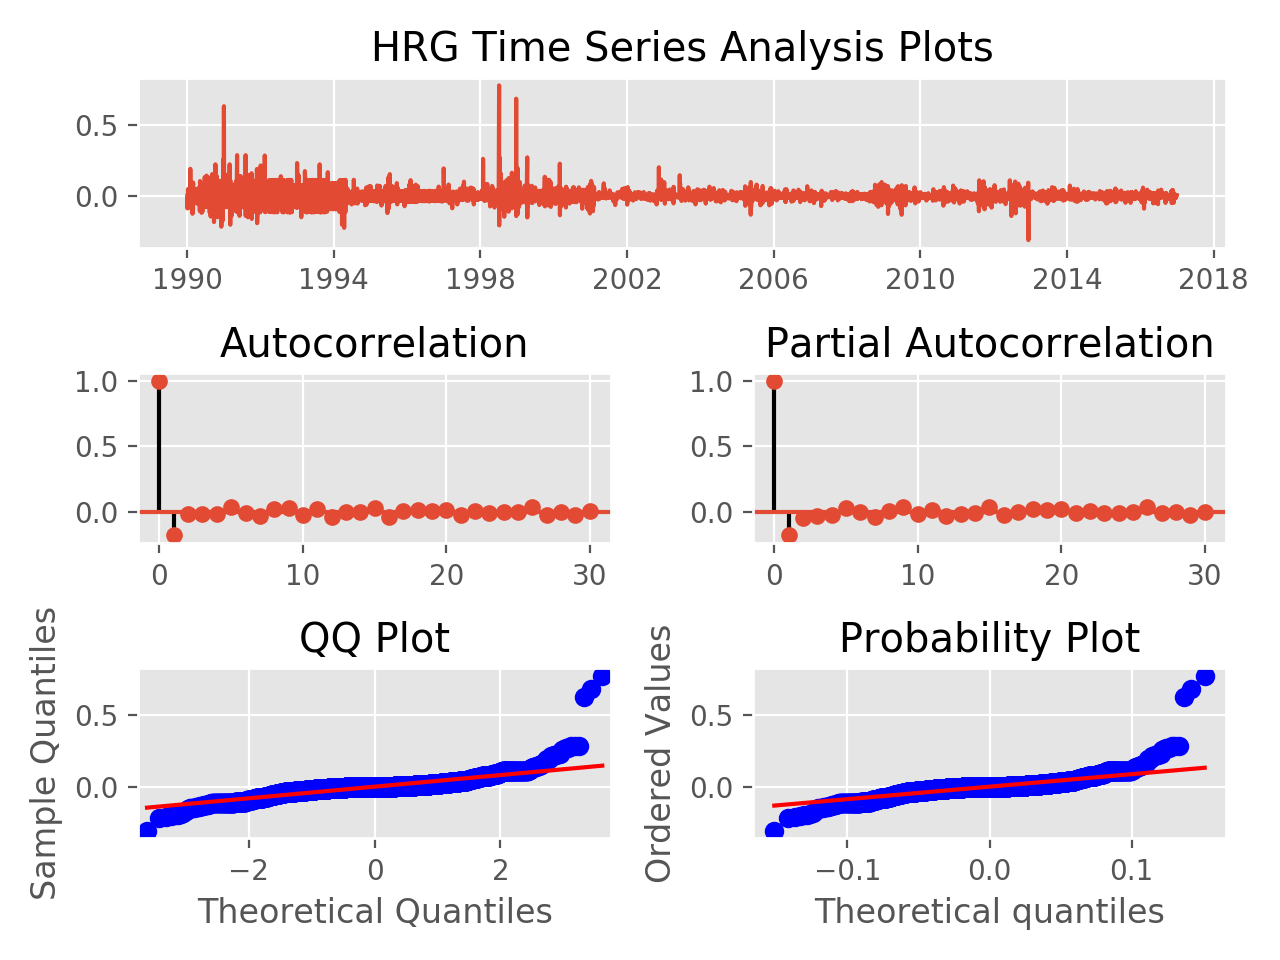
\includegraphics[width=\textwidth]{HRG-time-series.png}
\includegraphics[width=\textwidth]{HRG-histogram.png}
\includegraphics[width=\textwidth]{HL-time-series.png}
\includegraphics[width=\textwidth]{HL-histogram.png}

\subsection{Ordinary Least Squares (OLS)}
MSFT scored a mean absolute error regression loss of 0.810, and a coefficient of determination of 0.991.

\includegraphics[width=\textwidth]{MSFT-OLS-In-Sample-Prediction.png}

\includegraphics[width=\textwidth]{100-Day-MSFT-OLS-Out-of-Sample-Forecast.png}

CDE scored a mean absolute error regression loss of 0.985, and a coefficient of determination of 0.973.

\includegraphics[width=\textwidth]{CDE-OLS-In-Sample-Prediction.png}

\includegraphics[width=\textwidth]{100-Day-CDE-OLS-Out-of-Sample-Forecast.png}

NAVB scored a mean absolute error regression loss of 0.124, and a coefficient of determination of 0.966.

\includegraphics[width=\textwidth]{NAVB-OLS-In-Sample-Prediction.png}

\includegraphics[width=\textwidth]{100-Day-NAVB-OLS-Out-of-Sample-Forecast.png}

HRG scored a mean absolute error regression loss of 0.291, and a coefficient of determination of 0.986.

\includegraphics[width=\textwidth]{HRG-OLS-In-Sample-Prediction.png}

\includegraphics[width=\textwidth]{100-Day-HRG-OLS-Out-of-Sample-Forecast.png}

HL scored a mean absolute error regression loss of 0.336, and a coefficient of determination of 0.963.

\includegraphics[width=\textwidth]{HL-OLS-In-Sample-Prediction.png}

\includegraphics[width=\textwidth]{100-Day-HL-OLS-Out-of-Sample-Forecast.png}

\subsection{Auto Regressive (AR)}
\includegraphics[width=\textwidth]{MSFT-AR-time-series.png}
\includegraphics[width=\textwidth]{MSFT-AR-histogram.png}
\includegraphics[width=\textwidth]{MSFT-AR-In-Sample-Return-Prediction.png}
\includegraphics[width=\textwidth]{100-Day-MSFT-AR-Out-of-Sample-Return-Forecast.png}
\includegraphics[width=\textwidth]{CDE-AR-time-series.png}
\includegraphics[width=\textwidth]{CDE-AR-histogram.png}
\includegraphics[width=\textwidth]{CDE-AR-In-Sample-Return-Prediction.png}
\includegraphics[width=\textwidth]{100-Day-CDE-AR-Out-of-Sample-Return-Forecast.png}
\includegraphics[width=\textwidth]{NAVB-AR-time-series.png}
\includegraphics[width=\textwidth]{NAVB-AR-histogram.png}
\includegraphics[width=\textwidth]{NAVB-AR-In-Sample-Return-Prediction.png}
\includegraphics[width=\textwidth]{100-Day-NAVB-AR-Out-of-Sample-Return-Forecast.png}
\includegraphics[width=\textwidth]{HRG-AR-time-series.png}
\includegraphics[width=\textwidth]{HRG-AR-histogram.png}
\includegraphics[width=\textwidth]{HRG-AR-In-Sample-Return-Prediction.png}
\includegraphics[width=\textwidth]{100-Day-HRG-AR-Out-of-Sample-Return-Forecast.png}
\includegraphics[width=\textwidth]{HL-AR-time-series.png}
\includegraphics[width=\textwidth]{HL-AR-histogram.png}
\includegraphics[width=\textwidth]{HL-AR-In-Sample-Return-Prediction.png}
\includegraphics[width=\textwidth]{100-Day-HL-AR-Out-of-Sample-Return-Forecast.png}

\subsection{Moving Average (MA)}
\includegraphics[width=\textwidth]{MSFT-MA-time-series.png}
\includegraphics[width=\textwidth]{MSFT-MA-histogram.png}
\includegraphics[width=\textwidth]{MSFT-MA-In-Sample-Return-Prediction.png}
\includegraphics[width=\textwidth]{100-Day-MSFT-MA-Out-of-Sample-Return-Forecast.png}
\includegraphics[width=\textwidth]{CDE-MA-time-series.png}
\includegraphics[width=\textwidth]{CDE-MA-histogram.png}
\includegraphics[width=\textwidth]{CDE-MA-In-Sample-Return-Prediction.png}
\includegraphics[width=\textwidth]{100-Day-CDE-MA-Out-of-Sample-Return-Forecast.png}
\includegraphics[width=\textwidth]{NAVB-MA-time-series.png}
\includegraphics[width=\textwidth]{NAVB-MA-histogram.png}
\includegraphics[width=\textwidth]{NAVB-MA-In-Sample-Return-Prediction.png}
\includegraphics[width=\textwidth]{100-Day-NAVB-MA-Out-of-Sample-Return-Forecast.png}
\includegraphics[width=\textwidth]{HRG-MA-time-series.png}
\includegraphics[width=\textwidth]{HRG-MA-histogram.png}
\includegraphics[width=\textwidth]{HRG-MA-In-Sample-Return-Prediction.png}
\includegraphics[width=\textwidth]{100-Day-HRG-MA-Out-of-Sample-Return-Forecast.png}
\includegraphics[width=\textwidth]{HL-MA-time-series.png}
\includegraphics[width=\textwidth]{HL-MA-histogram.png}
\includegraphics[width=\textwidth]{HL-MA-In-Sample-Return-Prediction.png}
\includegraphics[width=\textwidth]{100-Day-HL-MA-Out-of-Sample-Return-Forecast.png}

\subsection{Auto Regressive Moving Average (ARMA)}
\includegraphics[width=\textwidth]{MSFT-ARMA-time-series.png}
\includegraphics[width=\textwidth]{MSFT-ARMA-histogram.png}
\includegraphics[width=\textwidth]{MSFT-ARMA-In-Sample-Return-Prediction.png}
\includegraphics[width=\textwidth]{100-Day-MSFT-ARMA-Out-of-Sample-Return-Forecast.png}
\includegraphics[width=\textwidth]{CDE-ARMA-time-series.png}
\includegraphics[width=\textwidth]{CDE-ARMA-histogram.png}
\includegraphics[width=\textwidth]{CDE-ARMA-In-Sample-Return-Prediction.png}
\includegraphics[width=\textwidth]{100-Day-CDE-ARMA-Out-of-Sample-Return-Forecast.png}
\includegraphics[width=\textwidth]{NAVB-ARMA-time-series.png}
\includegraphics[width=\textwidth]{NAVB-ARMA-histogram.png}
\includegraphics[width=\textwidth]{NAVB-ARMA-In-Sample-Return-Prediction.png}
\includegraphics[width=\textwidth]{100-Day-NAVB-ARMA-Out-of-Sample-Return-Forecast.png}
\includegraphics[width=\textwidth]{HRG-ARMA-time-series.png}
\includegraphics[width=\textwidth]{HRG-ARMA-histogram.png}
\includegraphics[width=\textwidth]{HRG-ARMA-In-Sample-Return-Prediction.png}
\includegraphics[width=\textwidth]{100-Day-HRG-ARMA-Out-of-Sample-Return-Forecast.png}
\includegraphics[width=\textwidth]{HL-ARMA-time-series.png}
\includegraphics[width=\textwidth]{HL-ARMA-histogram.png}
\includegraphics[width=\textwidth]{HL-ARMA-In-Sample-Return-Prediction.png}
\includegraphics[width=\textwidth]{100-Day-HL-ARMA-Out-of-Sample-Return-Forecast.png}

\subsection{Auto Regressive Integrated Moving Average (ARIMA)}
\includegraphics[width=\textwidth]{MSFT-ARIMA-time-series.png}
\includegraphics[width=\textwidth]{MSFT-ARIMA-histogram.png}
\includegraphics[width=\textwidth]{MSFT-ARIMA-In-Sample-Return-Prediction.png}
\includegraphics[width=\textwidth]{100-Day-MSFT-ARIMA-Out-of-Sample-Return-Forecast.png}
\includegraphics[width=\textwidth]{CDE-ARIMA-time-series.png}
\includegraphics[width=\textwidth]{CDE-ARIMA-histogram.png}
\includegraphics[width=\textwidth]{CDE-ARIMA-In-Sample-Return-Prediction.png}
\includegraphics[width=\textwidth]{100-Day-CDE-ARIMA-Out-of-Sample-Return-Forecast.png}
\includegraphics[width=\textwidth]{NAVB-ARIMA-time-series.png}
\includegraphics[width=\textwidth]{NAVB-ARIMA-histogram.png}
\includegraphics[width=\textwidth]{NAVB-ARIMA-In-Sample-Return-Prediction.png}
\includegraphics[width=\textwidth]{100-Day-NAVB-ARIMA-Out-of-Sample-Return-Forecast.png}
\includegraphics[width=\textwidth]{HRG-ARIMA-time-series.png}
\includegraphics[width=\textwidth]{HRG-ARIMA-histogram.png}
\includegraphics[width=\textwidth]{HRG-ARIMA-In-Sample-Return-Prediction.png}
\includegraphics[width=\textwidth]{100-Day-HRG-ARIMA-Out-of-Sample-Return-Forecast.png}
\includegraphics[width=\textwidth]{HL-ARIMA-time-series.png}
\includegraphics[width=\textwidth]{HL-ARIMA-histogram.png}
\includegraphics[width=\textwidth]{HL-ARIMA-In-Sample-Return-Prediction.png}
\includegraphics[width=\textwidth]{100-Day-HL-ARIMA-Out-of-Sample-Return-Forecast.png}

\section{Machine Learning}

\subsection{Classification}

\subsubsection{Decision Tree}

\begin{center}
    \begin{tabular}{ | l | l | l | | l | l | l | p{5cm} |}
    \hline
    Ticker & Precision & True Negatives & False Negatives & True Positives & False Positives \\ \hline
    MSFT & 0.77 & 493 & 131 & 547 & 190 \\ \hline
    CDE & 0.79 & 565 & 144 & 504 & 133 \\ \hline
    NAVB & 0.76 & 592 & 165 & 331 & 126 \\ \hline
    HRG & 0.75 & 553 & 210 & 462 & 135 \\ \hline
    HL & 0.79 & 603 & 135 & 475 & 147 \\
    \hline
    \end{tabular}
\end{center}

\subsubsection{Boosted Decision Tree}

\begin{center}
    \begin{tabular}{ | l | l | l | | l | l | l | p{5cm} |}
    \hline
    Ticker & Precision & True Negatives & False Negatives & True Positives & False Positives \\ \hline
    MSFT & 0.77 & 493 & 130 & 548 & 190 \\ \hline
    CDE & 0.79 & 564 & 143 & 505 & 134 \\ \hline
    NAVB & 0.76 & 588 & 164 & 332 & 130 \\ \hline
    HRG & 0.75 & 542 & 191 & 481 & 146 \\ \hline
    HL & 0.79 & 602 & 132 & 478 & 149 \\
    \hline
    \end{tabular}
\end{center}

\subsubsection{Support Vector Machine (SVM)}

\begin{center}
    \begin{tabular}{ | l | l | l | | l | l | l | p{5cm} |}
    \hline
    Ticker & Precision & True Negatives & False Negatives & True Positives & False Positives \\ \hline
    MSFT & 0.77 & 493 & 130 & 548 & 190 \\ \hline
    CDE & 0.79 & 564 & 143 & 505 & 134 \\ \hline
    NAVB & 0.76 & 593 & 169 & 327 & 125 \\ \hline
    HRG & 0.75 & 542 & 191 & 481 & 146 \\ \hline
    HL & 0.81 & 579 & 98 & 512 & 171 \\
    \hline
    \end{tabular}
\end{center}

\subsubsection{Random Forest}

\begin{center}
    \begin{tabular}{ | l | l | l | | l | l | l | p{5cm} |}
    \hline
    Ticker & Precision & True Negatives & False Negatives & True Positives & False Positives \\ \hline
    MSFT & 0.77 & 493 & 131 & 547 & 190 \\ \hline
    CDE & 0.79 & 566 & 145 & 503 & 132 \\ \hline
    NAVB & 0.76 & 590 & 164 & 332 & 128 \\ \hline
    HRG & 0.75 & 554 & 210 & 462 & 134 \\ \hline
    HL & 0.81 & 581 & 101 & 509 & 169 \\
    \hline
    \end{tabular}
\end{center}

\subsubsection{K-Nearest Neighbour}

\begin{center}
    \begin{tabular}{ | l | l | l | | l | l | l | p{5cm} |}
    \hline
    Ticker & Precision & True Negatives & False Negatives & True Positives & False Positives \\ \hline
    MSFT & 0.76 & 489 & 130 & 548 & 194 \\ \hline
    CDE & 0.80 & 574 & 147 & 501 & 126 \\ \hline
    NAVB & 0.75 & 573 & 161 & 335 & 145 \\ \hline
    HRG & 0.74 & 560 & 233 & 439 & 128 \\ \hline
    HL & 0.81 & 581 & 101 & 509 & 169 \\
    \hline
    \end{tabular}
\end{center}

\subsubsection{Gaussian Naive Bayes}

\begin{center}
    \begin{tabular}{ | l | l | l | | l | l | l | p{5cm} |}
    \hline
    Ticker & Precision & True Negatives & False Negatives & True Positives & False Positives \\ \hline
    MSFT & 0.73 & 478 & 168 & 510 & 205 \\ \hline
    CDE & 0.76 & 555 & 187 & 461 & 143 \\ \hline
    NAVB & 0.74 & 553 & 153 & 343 & 165 \\ \hline
    HRG & 0.73 & 491 & 170 & 502 & 197 \\ \hline
    HL & 0.77 & 590 & 157 & 453 & 160 \\
    \hline
    \end{tabular}
\end{center}

\subsubsection{Bernoulli Naive Bayes}

\begin{center}
    \begin{tabular}{ | l | l | l | | l | l | l | p{5cm} |}
    \hline
    Ticker & Precision & True Negatives & False Negatives & True Positives & False Positives \\ \hline
    MSFT & 0.73 & 479 & 169 & 509 & 204 \\ \hline
    CDE & 0.76 & 558 & 187 & 461 & 140 \\ \hline
    NAVB & 0.74 & 553 & 153 & 343 & 165 \\ \hline
    HRG & 0.73 & 492 & 170 & 502 & 196 \\ \hline
    HL & 0.77 & 590 & 158 & 452 & 160 \\
    \hline
    \end{tabular}
\end{center}

\subsubsection{Neural Network}

\begin{center}
    \begin{tabular}{ | l | l | l | | l | l | l | p{5cm} |}
    \hline
    Ticker & Precision & True Negatives & False Negatives & True Positives & False Positives \\ \hline
    MSFT & 0.77 & 685 & 181 & 787 & 258 \\ \hline
    CDE & 0.79 & 616 & 156 & 542 & 152 \\ \hline
    NAVB & 0.76 & 691 & 183 & 403 & 153 \\ \hline
    HRG & 0.74 & 690 & 269 & 542 & 164 \\ \hline
    HL & 0.77 & 1059 & 270 & 848 & 164 \\
    \hline
    \end{tabular}
\end{center}

\subsubsection{Logistic Regression}

\begin{center}
    \begin{tabular}{ | l | l | l | | l | l | l | p{5cm} |}
    \hline
    Ticker & Precision & True Negatives & False Negatives & True Positives & False Positives \\ \hline
    MSFT & 0.77 & 493 & 130 & 548 & 190 \\ \hline
    CDE & 0.79 & 564 & 143 & 505 & 134 \\ \hline
    NAVB & 0.76 & 588 & 164 & 332 & 130 \\ \hline
    HRG & 0.75 & 542 & 191 & 481 & 146 \\ \hline
    HL & 0.79 & 601 & 132 & 478 & 149 \\
    \hline
    \end{tabular}
\end{center}

\subsubsection{Stochastic Gradient Descent}

\begin{center}
    \begin{tabular}{ | l | l | l | | l | l | l | p{5cm} |}
    \hline
    Ticker & Precision & True Negatives & False Negatives & True Positives & False Positives \\ \hline
    MSFT & 0.77 & 493 & 130 & 548 & 190 \\ \hline
    CDE & 0.76 & 462 & 106 & 542 & 236 \\ \hline
    NAVB & 0.59 & 1032 & 707 & 118 & 80 \\ \hline
    HRG & 0.72 & 761 & 225 & 1059 & 518 \\ \hline
    HL & 0.80 & 535 & 83 & 527 & 215 \\
    \hline
    \end{tabular}
\end{center}

\subsection{Regression}

\subsubsection{Decision Tree}
MSFT scored a mean absolute error regression loss of 5.606, and a coefficient of determination of 0.458.

\includegraphics[width=\textwidth]{MSFT-Decision-Trees-In-Sample-Prediction.png}

\includegraphics[width=\textwidth]{100-Day-MSFT-Decision-Trees-Out-of-Sample-Forecast.png}

CDE scored a mean absolute error regression loss of 2.906, and a coefficient of determination of 0.816.

\includegraphics[width=\textwidth]{CDE-Decision-Trees-In-Sample-Prediction.png}

\includegraphics[width=\textwidth]{100-Day-CDE-Decision-Trees-Out-of-Sample-Forecast.png}

NAVB scored a mean absolute error regression loss of 0.422, and a coefficient of determination of 0.693.

\includegraphics[width=\textwidth]{NAVB-Decision-Trees-In-Sample-Prediction.png}

\includegraphics[width=\textwidth]{100-Day-NAVB-Decision-Trees-Out-of-Sample-Forecast.png}

HRG scored a mean absolute error regression loss of 1.415, and a coefficient of determination of 0.464.

\includegraphics[width=\textwidth]{HRG-Decision-Trees-In-Sample-Prediction.png}

\includegraphics[width=\textwidth]{100-Day-HRG-Decision-Trees-Out-of-Sample-Forecast.png}

HL scored a mean absolute error regression loss of 0.506, and a coefficient of determination of 0.923.

\includegraphics[width=\textwidth]{HL-Decision-Trees-In-Sample-Prediction.png}

\includegraphics[width=\textwidth]{100-Day-HL-Decision-Trees-Out-of-Sample-Forecast.png}

\subsubsection{Boosted Decision Tree}
MSFT scored a mean absolute error regression loss of 4.426, and a coefficient of determination of 0.580.

\includegraphics[width=\textwidth]{MSFT-Boosted-Trees-In-Sample-Prediction.png}

\includegraphics[width=\textwidth]{100-Day-MSFT-Boosted-Trees-Out-of-Sample-Forecast.png}

CDE scored a mean absolute error regression loss of 5.452, and a coefficient of determination of 0.581.

\includegraphics[width=\textwidth]{CDE-Boosted-Trees-In-Sample-Prediction.png}

\includegraphics[width=\textwidth]{100-Day-CDE-Boosted-Trees-Out-of-Sample-Forecast.png}

NAVB scored a mean absolute error regression loss of 0.579, and a coefficient of determination of 0.509.

\includegraphics[width=\textwidth]{NAVB-Boosted-Trees-In-Sample-Prediction.png}

\includegraphics[width=\textwidth]{100-Day-NAVB-Boosted-Trees-Out-of-Sample-Forecast.png}

HRG scored a mean absolute error regression loss of 0.980, and a coefficient of determination of 0.855.

\includegraphics[width=\textwidth]{HRG-Boosted-Trees-In-Sample-Prediction.png}

\includegraphics[width=\textwidth]{100-Day-HRG-Boosted-Trees-Out-of-Sample-Forecast.png}

HL scored a mean absolute error regression loss of 0.410, and a coefficient of determination of 0.952.

\includegraphics[width=\textwidth]{HL-Boosted-Trees-In-Sample-Prediction.png}

\includegraphics[width=\textwidth]{100-Day-HL-Boosted-Trees-Out-of-Sample-Forecast.png}

\subsubsection{K-Nearest Neighbour}
MSFT scored a mean absolute error regression loss of 4.426, and a coefficient of determination of 0.580.

\includegraphics[width=\textwidth]{MSFT-K-Nearest-Neighbour-In-Sample-Prediction.png}

\includegraphics[width=\textwidth]{100-Day-MSFT-K-Nearest-Neighbour-Out-of-Sample-Forecast.png}

CDE scored a mean absolute error regression loss of 5.452, and a coefficient of determination of 0.581.

\includegraphics[width=\textwidth]{CDE-K-Nearest-Neighbour-In-Sample-Prediction.png}

\includegraphics[width=\textwidth]{100-Day-CDE-K-Nearest-Neighbour-Out-of-Sample-Forecast.png}

NAVB scored a mean absolute error regression loss of 0.579, and a coefficient of determination of 0.509.

\includegraphics[width=\textwidth]{NAVB-K-Nearest-Neighbour-In-Sample-Prediction.png}

\includegraphics[width=\textwidth]{100-Day-NAVB-K-Nearest-Neighbour-Out-of-Sample-Forecast.png}

HRG scored a mean absolute error regression loss of 0.980, and a coefficient of determination of 0.855.

\includegraphics[width=\textwidth]{HRG-K-Nearest-Neighbour-In-Sample-Prediction.png}

\includegraphics[width=\textwidth]{100-Day-HRG-K-Nearest-Neighbour-Out-of-Sample-Forecast.png}

HL scored a mean absolute error regression loss of 0.410, and a coefficient of determination of 0.952.

\includegraphics[width=\textwidth]{HL-K-Nearest-Neighbour-In-Sample-Prediction.png}

\includegraphics[width=\textwidth]{100-Day-HL-K-Nearest-Neighbour-Out-of-Sample-Forecast.png}

\subsubsection{Random Forest}
MSFT scored a mean absolute error regression loss of 5.199, and a coefficient of determination of 0.483.

\includegraphics[width=\textwidth]{MSFT-Random-Forest-In-Sample-Prediction.png}

\includegraphics[width=\textwidth]{100-Day-MSFT-Random-Forest-Out-of-Sample-Forecast.png}

CDE scored a mean absolute error regression loss of 2.505, and a coefficient of determination of 0.861.

\includegraphics[width=\textwidth]{CDE-Random-Forest-In-Sample-Prediction.png}

\includegraphics[width=\textwidth]{100-Day-CDE-Random-Forest-Out-of-Sample-Forecast.png}

NAVB scored a mean absolute error regression loss of 0.293, and a coefficient of determination of 0.856.

\includegraphics[width=\textwidth]{NAVB-Random-Forest-In-Sample-Prediction.png}

\includegraphics[width=\textwidth]{100-Day-NAVB-Random-Forest-Out-of-Sample-Forecast.png}

HRG scored a mean absolute error regression loss of 0.675, and a coefficient of determination of 0.907.

\includegraphics[width=\textwidth]{HRG-Random-Forest-In-Sample-Prediction.png}

\includegraphics[width=\textwidth]{100-Day-HRG-Random-Forest-Out-of-Sample-Forecast.png}

HL scored a mean absolute error regression loss of 0.434, and a coefficient of determination of 0.922.

\includegraphics[width=\textwidth]{HL-Random-Forest-In-Sample-Prediction.png}

\includegraphics[width=\textwidth]{100-Day-HL-Random-Forest-Out-of-Sample-Forecast.png}

\subsubsection{Linear Regression}
MSFT scored a mean absolute error regression loss of 0.844, and a coefficient of determination of 0.990.

\includegraphics[width=\textwidth]{MSFT-Linear-Regression-In-Sample-Prediction.png}

\includegraphics[width=\textwidth]{100-Day-MSFT-Linear-Regression-Out-of-Sample-Forecast.png}

CDE scored a mean absolute error regression loss of 0.990, and a coefficient of determination of 0.972.

\includegraphics[width=\textwidth]{CDE-Linear-Regression-In-Sample-Prediction.png}

\includegraphics[width=\textwidth]{100-Day-CDE-Linear-Regression-Out-of-Sample-Forecast.png}

NAVB scored a mean absolute error regression loss of 0.128, and a coefficient of determination of 0.962.

\includegraphics[width=\textwidth]{NAVB-Linear-Regression-In-Sample-Prediction.png}

\includegraphics[width=\textwidth]{100-Day-NAVB-Linear-Regression-Out-of-Sample-Forecast.png}

HRG scored a mean absolute error regression loss of 0.324, and a coefficient of determination of 0.984.

\includegraphics[width=\textwidth]{HRG-Linear-Regression-In-Sample-Prediction.png}

\includegraphics[width=\textwidth]{100-Day-HRG-Linear-Regression-Out-of-Sample-Forecast.png}

HL scored a mean absolute error regression loss of 0.243, and a coefficient of determination of 0.964.

\includegraphics[width=\textwidth]{HL-Linear-Regression-In-Sample-Prediction.png}

\includegraphics[width=\textwidth]{100-Day-HL-Linear-Regression-Out-of-Sample-Forecast.png}

\subsubsection{Neural Network}
MSFT scored a mean absolute error regression loss of 1.073, and a coefficient of determination of 0.992.

\includegraphics[width=\textwidth]{MSFT-Neural-Network-In-Sample-Prediction.png}

\includegraphics[width=\textwidth]{100-Day-MSFT-Neural-Network-Out-of-Sample-Forecast.png}

CDE scored a mean absolute error regression loss of 2.906, and a coefficient of determination of 0.816.

\includegraphics[width=\textwidth]{CDE-Neural-Network-In-Sample-Prediction.png}

\includegraphics[width=\textwidth]{100-Day-CDE-Neural-Network-Out-of-Sample-Forecast.png}

NAVB scored a mean absolute error regression loss of 0.422, and a coefficient of determination of 0.693.

\includegraphics[width=\textwidth]{NAVB-Neural-Network-In-Sample-Prediction.png}

\includegraphics[width=\textwidth]{100-Day-NAVB-Neural-Network-Out-of-Sample-Forecast.png}

HRG scored a mean absolute error regression loss of 1.415, and a coefficient of determination of 0.464.

\includegraphics[width=\textwidth]{HRG-Neural-Network-In-Sample-Prediction.png}

\includegraphics[width=\textwidth]{100-Day-HRG-Neural-Network-Out-of-Sample-Forecast.png}

HL scored a mean absolute error regression loss of 0.506, and a coefficient of determination of 0.923.

\includegraphics[width=\textwidth]{HL-Neural-Network-In-Sample-Prediction.png}

\includegraphics[width=\textwidth]{100-Day-HL-Neural-Network-Out-of-Sample-Forecast.png}

\subsubsection{Stochastic Gradient Descent}
MSFT scored a mean absolute error regression loss of 0.829, and a coefficient of determination of 0.990.

\includegraphics[width=\textwidth]{MSFT-SGD-In-Sample-Prediction.png}

\includegraphics[width=\textwidth]{100-Day-MSFT-SGD-Out-of-Sample-Forecast.png}

CDE scored a mean absolute error regression loss of 4.724, and a coefficient of determination of 0.788.

\includegraphics[width=\textwidth]{CDE-SGD-In-Sample-Prediction.png}

\includegraphics[width=\textwidth]{100-Day-CDE-SGD-Out-of-Sample-Forecast.png}

NAVB scored a mean absolute error regression loss of 0.142, and a coefficient of determination of 0.955.

\includegraphics[width=\textwidth]{NAVB-SGD-In-Sample-Prediction.png}

\includegraphics[width=\textwidth]{100-Day-NAVB-SGD-Out-of-Sample-Forecast.png}

HRG scored a mean absolute error regression loss of 0.292, and a coefficient of determination of 0.987.

\includegraphics[width=\textwidth]{HRG-SGD-In-Sample-Prediction.png}

\includegraphics[width=\textwidth]{100-Day-HRG-SGD-Out-of-Sample-Forecast.png}

HL scored a mean absolute error regression loss of 0.275, and a coefficient of determination of 0.962.

\includegraphics[width=\textwidth]{HL-SGD-In-Sample-Prediction.png}

\includegraphics[width=\textwidth]{100-Day-HL-SGD-Out-of-Sample-Forecast.png}

\section{Bayesian Statistics}

\subsection{No-U-Turn Sampler (NUTS)}
MSFT scored a mean absolute error regression loss of 5.606, and a coefficient of determination of 0.458.

\includegraphics[width=\textwidth]{MSFT-NUTS-In-Sample-Returns-Prediction.png}

\includegraphics[width=\textwidth]{100-Day-MSFT-NUTS-Out-of-Sample-Returns-Forecast.png}

CDE scored a mean absolute error regression loss of 2.906, and a coefficient of determination of 0.816.

\includegraphics[width=\textwidth]{CDE-NUTS-In-Sample-Returns-Prediction.png}

\includegraphics[width=\textwidth]{100-Day-CDE-NUTS-Out-of-Sample-Returns-Forecast.png}

NAVB scored a mean absolute error regression loss of 0.422, and a coefficient of determination of 0.693.

\includegraphics[width=\textwidth]{NAVB-NUTS-In-Sample-Returns-Prediction.png}

\includegraphics[width=\textwidth]{100-Day-NAVB-NUTS-Out-of-Sample-Returns-Forecast.png}

HRG scored a mean absolute error regression loss of 1.415, and a coefficient of determination of 0.464.

\includegraphics[width=\textwidth]{HRG-NUTS-In-Sample-Returns-Prediction.png}

\includegraphics[width=\textwidth]{100-Day-HRG-NUTS-Out-of-Sample-Returns-Forecast.png}

HL scored a mean absolute error regression loss of 0.506, and a coefficient of determination of 0.923.

\includegraphics[width=\textwidth]{HL-NUTS-In-Sample-Returns-Prediction.png}

\includegraphics[width=\textwidth]{100-Day-HL-NUTS-Out-of-Sample-Returns-Forecast.png}

\subsection{Metropolis-Hastings}
MSFT scored a mean absolute error regression loss of 5.606, and a coefficient of determination of 0.458.

\includegraphics[width=\textwidth]{MSFT-Metropolis-In-Sample-Returns-Prediction.png}

\includegraphics[width=\textwidth]{100-Day-MSFT-Metropolis-Out-of-Sample-Returns-Forecast.png}

CDE scored a mean absolute error regression loss of 2.906, and a coefficient of determination of 0.816.

\includegraphics[width=\textwidth]{CDE-Metropolis-In-Sample-Returns-Prediction.png}

\includegraphics[width=\textwidth]{100-Day-CDE-Metropolis-Out-of-Sample-Returns-Forecast.png}

NAVB scored a mean absolute error regression loss of 0.422, and a coefficient of determination of 0.693.

\includegraphics[width=\textwidth]{NAVB-Metropolis-In-Sample-Returns-Prediction.png}

\includegraphics[width=\textwidth]{100-Day-NAVB-Metropolis-Out-of-Sample-Returns-Forecast.png}

HRG scored a mean absolute error regression loss of 1.415, and a coefficient of determination of 0.464.

\includegraphics[width=\textwidth]{HRG-Metropolis-In-Sample-Returns-Prediction.png}

\includegraphics[width=\textwidth]{100-Day-HRG-Metropolis-Out-of-Sample-Returns-Forecast.png}

HL scored a mean absolute error regression loss of 0.506, and a coefficient of determination of 0.923.

\includegraphics[width=\textwidth]{HL-Metropolis-In-Sample-Returns-Prediction.png}

\includegraphics[width=\textwidth]{100-Day-HL-Metropolis-Out-of-Sample-Returns-Forecast.png}

\section{Strategy}

\subsection{Classification}

\includegraphics[width=\textwidth]{MLC-Portfolio-Benchmark.png}

\subsection{Regression}

\includegraphics[width=\textwidth]{MLR-Portfolio-Benchmark.png}